\documentclass[11pt]{article}
\usepackage{latexsym}
\usepackage{fancyhdr}
\usepackage{amssymb,amsmath,amsthm}
\usepackage[pdftex]{graphicx}
\usepackage[margin=1in]{geometry}


% Create answer counter to keep track of seperate responses
\newcounter{AnswerCounter}
\newcounter{SubAnswerCounter}
\setcounter{AnswerCounter}{1}
\setcounter{SubAnswerCounter}{1}

% Create answer environment which uses counter
\newenvironment{answer}[0]{
  \setcounter{SubAnswerCounter}{1}
  \bigskip
  \textbf{Solution \arabic{AnswerCounter}}
  \\
  \begin{small}
}{
  \end{small}
  \stepcounter{AnswerCounter}
}

\newenvironment{subanswer}[0]{
  (\alph{SubAnswerCounter})
}{
 \bigskip
  \stepcounter{SubAnswerCounter}
}

% Custom Header information on each page
\pagestyle{fancy}
\lhead{HUID: 70871564}
\rhead{CS182: Luis APerez}
\renewcommand{\headrulewidth}{0.1pt}
\renewcommand{\footrulewidth}{0.1pt}

% Title page is page 0
\setcounter{page}{0}

\begin{document}
\begin{answer}[Problem 5]
We analyze the performance of CSP with forward checking and ordering.
\begin{table}[!h]
\centering
\caption{Node expansion and time comparison of heuristics for CSP.}
\label{tab:CSP_analysis}
\begin{tabular}{|l|l|l|l|l|}
\hline
                             & Time Elapsed  & Time Elapsed & Success Rate & Constraints Violated \\ \hline
Standard                     & 4.5712800026  & 56446        & N/A          & 0                    \\ \hline
Standard + Order0            & 11.1637690067 & 35200        & N/A          & 0                    \\ \hline
ForwardChecking              & 3.1771168709  & 6933         & N/A          & 0                    \\ \hline
ForwardChecking + Order      & 4.2519948483  & 4522         & N/A          & 0                    \\ \hline
Local Search (Easy, 5 times) & NA            & 6.859948349  & 20\%         & 4.2                  \\ \hline
Stochastic Local Search      & NA            & 4.552132082  & 80\%         & 0.4                  \\ \hline
\end{tabular}
\end{table}

As can be seen in Table \ref{tab:CSP_analysis}, the number of nodes expanded tended to decrease with both forward checking and ordering. In this regard, the algorithms improve. The improvement factor is actually quite significant. Adding order typically decreases the number of nodes explored by a factor of $2$, and using forward checking decreases the nodes explored by a factor of nearly $10$. Together, the two decrease the number of nodes expanded by over a factor of $10$.

Obviously, with a decrease in node expansion comes a decrease in time elapsed. However, it's interesting to note that adding order to the nodes typically increased the amount time elapsed. The most logical explanation for this is that while the nodes are now explored in a more optimal order, there's not much difference in small games of Sudoku between that order and the non-optimal order typically taken. Therefore, the time saved from exploring less nodes comes at the expense of even more time spent on each expansion as we attempt to figure out which node has the most restrictions.

Lastly, we can take a look at Figure \ref{fig:local} and Figure \ref{fig:stochastic} to see more detail about the local search. The optimization of randomly swapping even when the change is not an improvement helps immensely with the success rate. With stochastic descent, we have a success rate of $> 80\%$, while before the local search success rate was $<20\%$. We also see an improvement in the amount of time taken to solve the puzzle, though this is due mostly in part to the fact that less iterations are required if you stumble into a solution early on.

\begin{figure}[!h]
\centering
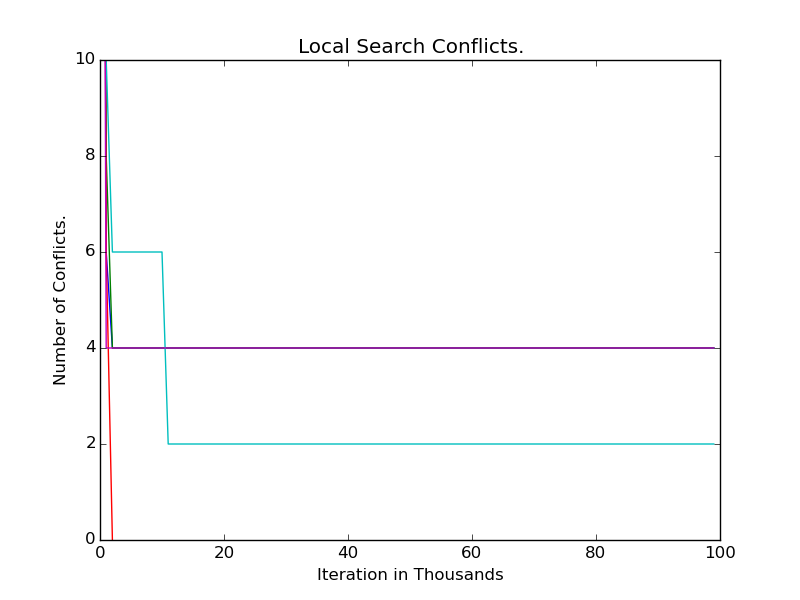
\includegraphics[scale=0.5]{local_search.png}
\caption{Local search without optimizations.}
\label{fig:local}
\end{figure}

\begin{figure}[!h]
\centering
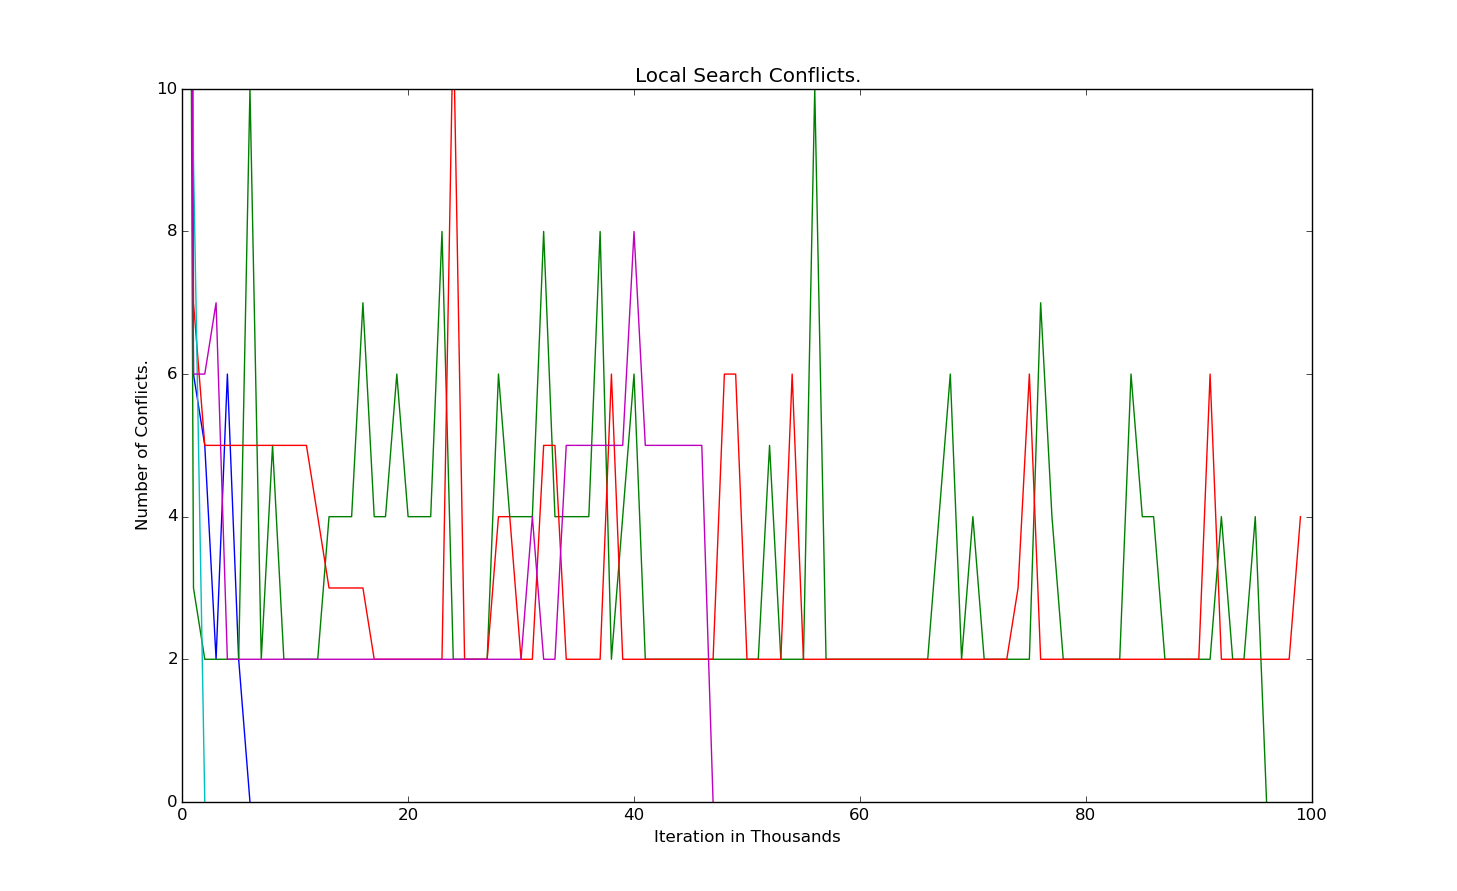
\includegraphics[scale=0.5]{stochastic_local_search.png}
\caption{Stochastic descent with $p = 0.01$ random movement.}
\label{fig:stochastic}
\end{figure}

\end{answer}
The design for a genetic algorithm that solves sudoku puzzles would be similar to our stochastic localized search. Initially, we'd generate a sequence of digits representing random entries (from $1$ to $9$) into empty slots (if we want to be clever, we do the same things as we did in local search and make sure we satisfy at least the row requirements) and have this represent a chromosome. We would measure fitness based on the inverse of the number of constraints violated for the given board (so that more violations give a lower fitness), with the likelihood of selection for mating equivalent to the normalized version over the population of this ``fitness'' score. For the cross over, we'd randomly select a location on the string to merge from each parent, with mutation consisting of the swapping of random elements on the same row. The algorithm would be similar to local search.
\begin{answer}[Problem 9]

\end{answer}
\end{document}